\documentclass{standalone}
\usepackage{tikz}
\usetikzlibrary{patterns, positioning}
\usepackage[sfdefault]{ClearSans} %% option 'sfdefault' activates Clear Sans as the default text font
\usepackage[T1]{fontenc}

\begin{document}
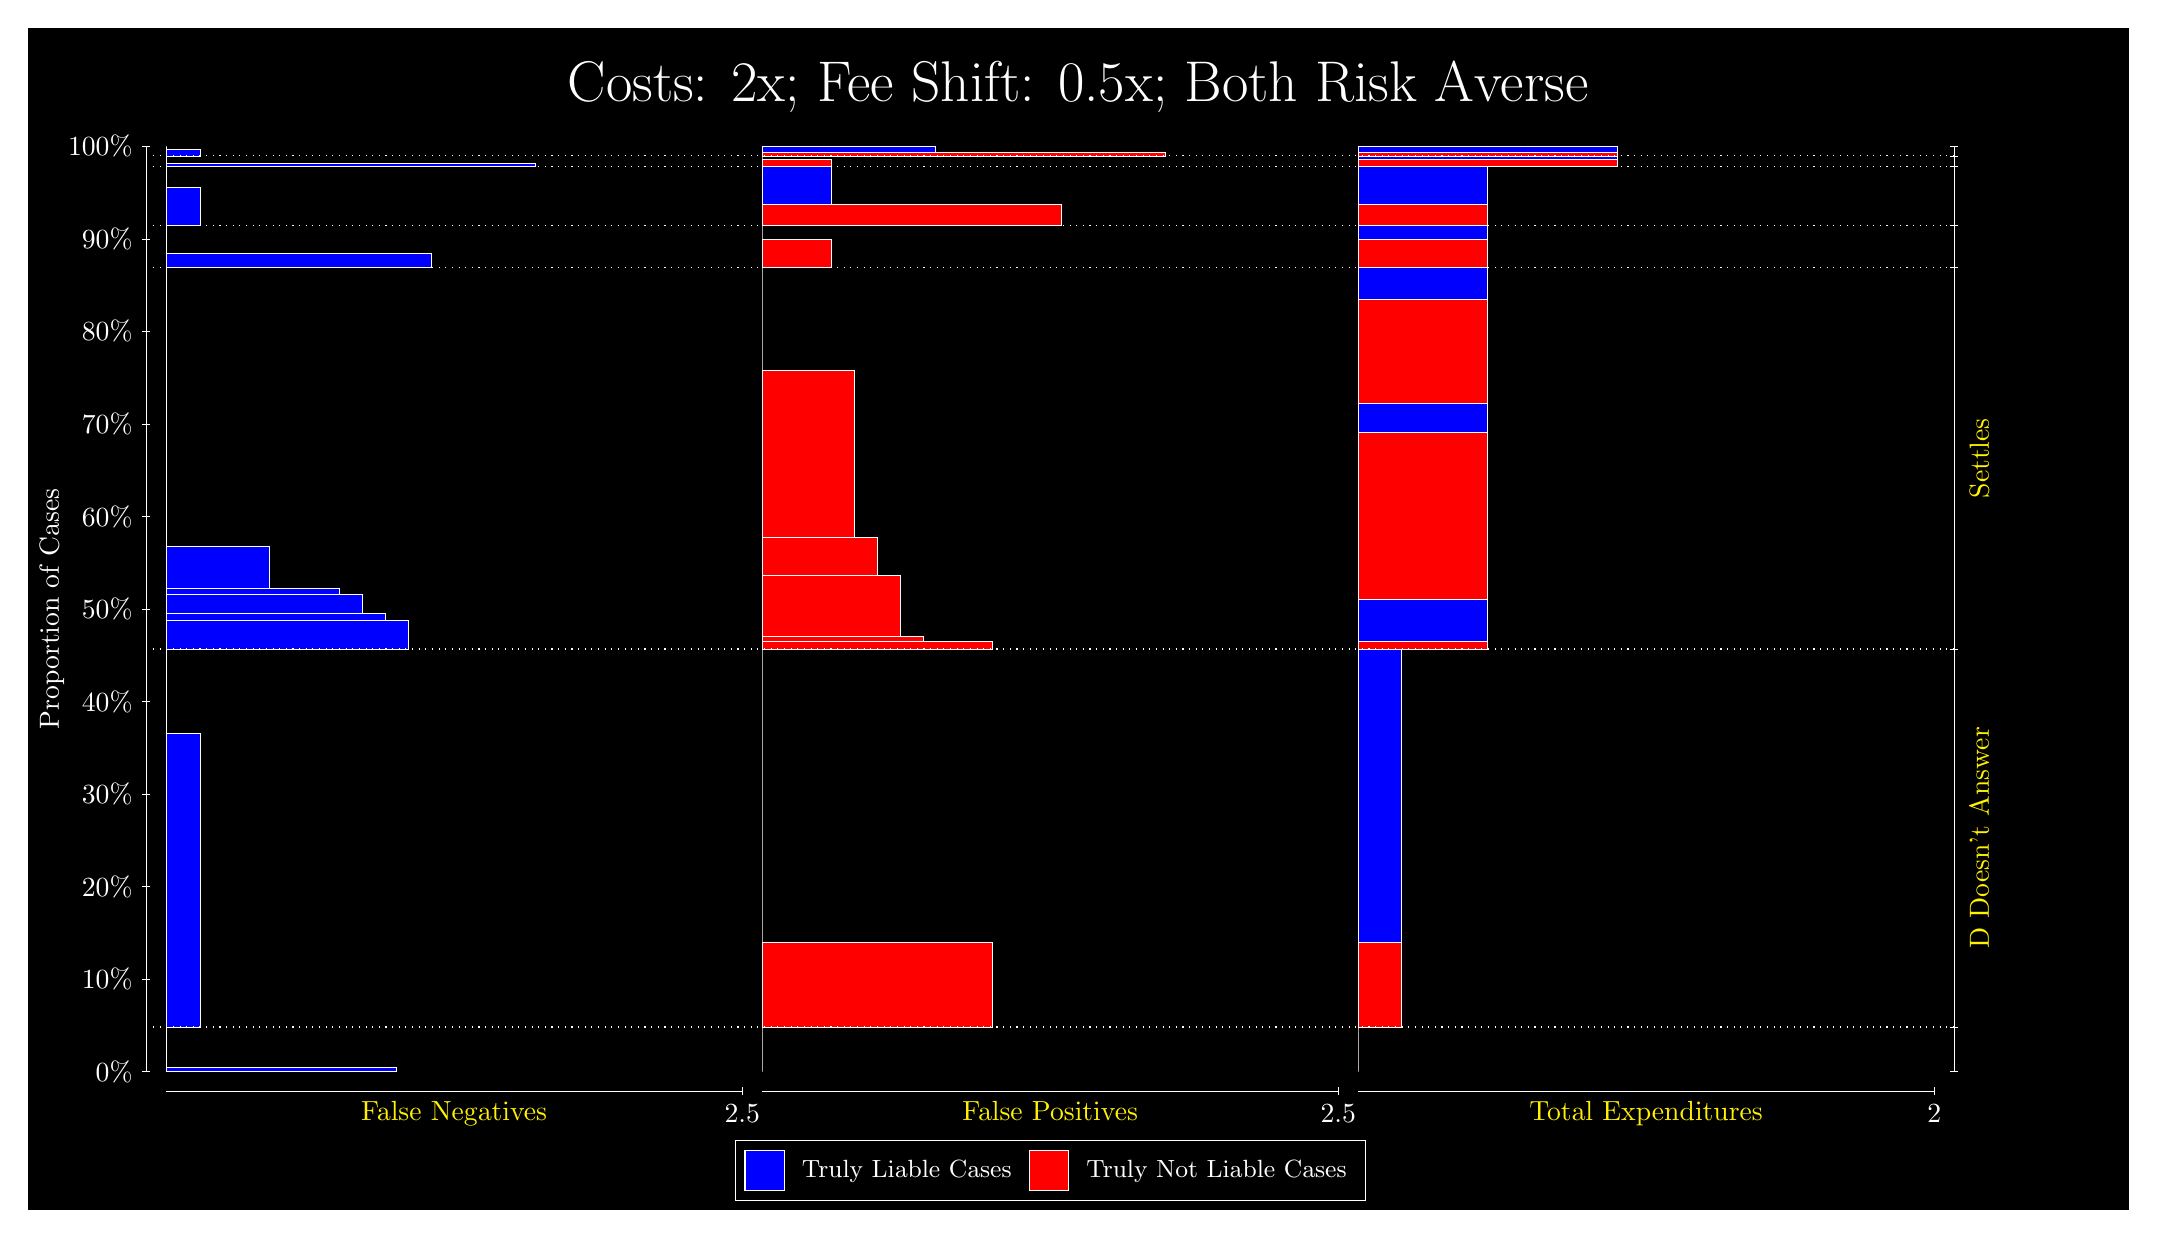
\begin{tikzpicture}
\draw[fill=black] (0,0) rectangle (26.667,15);
\draw[text=white] (0,13.5) rectangle (26.667,15) node[midway] {\huge Costs: 2x; Fee Shift: 0.5x; Both Risk Averse};
\draw[white, very thin] (1.5,1.75) -- (1.5,13.5);
\node[rotate=90, text=white, anchor=center] at (0.3, 7.625) {Proportion of Cases};
\draw[white, very thin] (1.45,1.75) -- (1.55,1.75);
\node[text=white, anchor=east] at (1.45, 1.75) {0\%};
\draw[white, very thin] (1.45,2.925) -- (1.55,2.925);
\node[text=white, anchor=east] at (1.45, 2.925) {10\%};
\draw[white, very thin] (1.45,4.1) -- (1.55,4.1);
\node[text=white, anchor=east] at (1.45, 4.1) {20\%};
\draw[white, very thin] (1.45,5.275) -- (1.55,5.275);
\node[text=white, anchor=east] at (1.45, 5.275) {30\%};
\draw[white, very thin] (1.45,6.45) -- (1.55,6.45);
\node[text=white, anchor=east] at (1.45, 6.45) {40\%};
\draw[white, very thin] (1.45,7.625) -- (1.55,7.625);
\node[text=white, anchor=east] at (1.45, 7.625) {50\%};
\draw[white, very thin] (1.45,8.8) -- (1.55,8.8);
\node[text=white, anchor=east] at (1.45, 8.8) {60\%};
\draw[white, very thin] (1.45,9.975) -- (1.55,9.975);
\node[text=white, anchor=east] at (1.45, 9.975) {70\%};
\draw[white, very thin] (1.45,11.15) -- (1.55,11.15);
\node[text=white, anchor=east] at (1.45, 11.15) {80\%};
\draw[white, very thin] (1.45,12.325) -- (1.55,12.325);
\node[text=white, anchor=east] at (1.45, 12.325) {90\%};
\draw[white, very thin] (1.45,13.5) -- (1.55,13.5);
\node[text=white, anchor=east] at (1.45, 13.5) {100\%};

\draw[white, very thin] (24.457,1.75) -- (24.457,13.5);
\draw[white, very thin] (24.407,1.75) -- (24.507,1.75);
\node[anchor=west] at (24.407, 1.75) {};
\draw[white, very thin] (24.407,2.3162) -- (24.507,2.3162);
\node[anchor=west] at (24.407, 2.3162) {};
\draw[white, very thin] (24.407,7.1164) -- (24.507,7.1164);
\node[anchor=west] at (24.407, 7.1164) {};
\draw[white, very thin] (24.407,11.963) -- (24.507,11.963);
\node[anchor=west] at (24.407, 11.963) {};
\draw[white, very thin] (24.407,12.493) -- (24.507,12.493);
\node[anchor=west] at (24.407, 12.493) {};
\draw[white, very thin] (24.407,13.248) -- (24.507,13.248);
\node[anchor=west] at (24.407, 13.248) {};
\draw[white, very thin] (24.407,13.378) -- (24.507,13.378);
\node[anchor=west] at (24.407, 13.378) {};
\draw[white, very thin] (24.407,13.5) -- (24.507,13.5);
\node[anchor=west] at (24.407, 13.5) {};

\draw[white, very thin, fill=blue] (1.75,1.75) rectangle (4.6775,1.8096);
\draw[white, very thin, fill=red] (1.75,1.8096) rectangle (1.75,2.3162);
\draw[white, very thin, fill=blue] (1.75,2.3162) rectangle (2.1891,6.0395);
\draw[white, very thin, fill=red] (1.75,6.0395) rectangle (1.75,7.1164);
\draw[white, very thin, fill=blue] (1.75,7.1164) rectangle (4.8239,7.4824);
\draw[white, very thin, fill=blue] (1.75,7.4824) rectangle (4.5312,7.5761);
\draw[white, very thin, fill=blue] (1.75,7.5761) rectangle (4.2384,7.81);
\draw[white, very thin, fill=blue] (1.75,7.81) rectangle (3.9457,7.886);
\draw[white, very thin, fill=blue] (1.75,7.886) rectangle (3.0674,8.4228);
\draw[white, very thin, fill=red] (1.75,8.4228) rectangle (1.75,11.963);
\draw[white, very thin, fill=blue] (1.75,11.963) rectangle (5.1167,12.142);
\draw[white, very thin, fill=red] (1.75,12.142) rectangle (1.75,12.493);
\draw[white, very thin, fill=blue] (1.75,12.493) rectangle (2.1891,12.978);
\draw[white, very thin, fill=red] (1.75,12.978) rectangle (1.75,13.248);
\draw[white, very thin, fill=blue] (1.75,13.248) rectangle (6.4341,13.289);
\draw[white, very thin, fill=red] (1.75,13.289) rectangle (1.75,13.378);
\draw[white, very thin, fill=blue] (1.75,13.378) rectangle (2.1891,13.459);
\draw[white, very thin, fill=red] (1.75,13.459) rectangle (1.75,13.5);
\draw[white, very thin, fill=red] (9.3189,1.75) rectangle (9.3189,2.2567);
\draw[white, very thin, fill=blue] (9.3189,2.2567) rectangle (9.3189,2.3162);
\draw[white, very thin, fill=red] (9.3189,2.3162) rectangle (12.246,3.3931);
\draw[white, very thin, fill=blue] (9.3189,3.3931) rectangle (9.3189,7.1164);
\draw[white, very thin, fill=red] (9.3189,7.1164) rectangle (12.246,7.2126);
\draw[white, very thin, fill=red] (9.3189,7.2126) rectangle (11.368,7.2739);
\draw[white, very thin, fill=red] (9.3189,7.2739) rectangle (11.075,8.0528);
\draw[white, very thin, fill=red] (9.3189,8.0528) rectangle (10.783,8.538);
\draw[white, very thin, fill=red] (9.3189,8.538) rectangle (10.49,10.657);
\draw[white, very thin, fill=blue] (9.3189,10.657) rectangle (9.3189,11.963);
\draw[white, very thin, fill=red] (9.3189,11.963) rectangle (10.197,12.314);
\draw[white, very thin, fill=blue] (9.3189,12.314) rectangle (9.3189,12.493);
\draw[white, very thin, fill=red] (9.3189,12.493) rectangle (13.125,12.763);
\draw[white, very thin, fill=blue] (9.3189,12.763) rectangle (10.197,13.248);
\draw[white, very thin, fill=red] (9.3189,13.248) rectangle (10.197,13.337);
\draw[white, very thin, fill=blue] (9.3189,13.337) rectangle (9.3189,13.378);
\draw[white, very thin, fill=red] (9.3189,13.378) rectangle (14.442,13.419);
\draw[white, very thin, fill=blue] (9.3189,13.419) rectangle (11.515,13.5);
\draw[white, very thin, fill=red] (16.888,1.75) rectangle (16.888,2.2567);
\draw[white, very thin, fill=blue] (16.888,2.2567) rectangle (16.888,2.3162);
\draw[white, very thin, fill=red] (16.888,2.3162) rectangle (17.437,3.3931);
\draw[white, very thin, fill=blue] (16.888,3.3931) rectangle (17.437,7.1164);
\draw[white, very thin, fill=red] (16.888,7.1164) rectangle (18.534,7.2126);
\draw[white, very thin, fill=blue] (16.888,7.2126) rectangle (18.534,7.7494);
\draw[white, very thin, fill=red] (16.888,7.7494) rectangle (18.534,9.8684);
\draw[white, very thin, fill=blue] (16.888,9.8684) rectangle (18.534,10.234);
\draw[white, very thin, fill=red] (16.888,10.234) rectangle (18.534,11.56);
\draw[white, very thin, fill=blue] (16.888,11.56) rectangle (18.534,11.963);
\draw[white, very thin, fill=red] (16.888,11.963) rectangle (18.534,12.314);
\draw[white, very thin, fill=blue] (16.888,12.314) rectangle (18.534,12.493);
\draw[white, very thin, fill=red] (16.888,12.493) rectangle (18.534,12.763);
\draw[white, very thin, fill=blue] (16.888,12.763) rectangle (18.534,13.248);
\draw[white, very thin, fill=red] (16.888,13.248) rectangle (20.181,13.337);
\draw[white, very thin, fill=blue] (16.888,13.337) rectangle (20.181,13.378);
\draw[white, very thin, fill=red] (16.888,13.378) rectangle (20.181,13.419);
\draw[white, very thin, fill=blue] (16.888,13.419) rectangle (20.181,13.5);
\draw[white, dotted] (1.5,2.3162) -- (24.457,2.3162);
\draw[white, dotted] (1.5,7.1164) -- (24.457,7.1164);
\draw[white, dotted] (1.5,11.963) -- (24.457,11.963);
\draw[white, dotted] (1.5,12.493) -- (24.457,12.493);
\draw[white, dotted] (1.5,13.248) -- (24.457,13.248);
\draw[white, dotted] (1.5,13.378) -- (24.457,13.378);
\draw[white, very thin] (1.75,1.5) -- (9.0689,1.5);
\node[text=yellow, anchor=north] at (5.4094, 1.5) {False Negatives};
\draw[white, very thin] (9.0689,1.45) -- (9.0689,1.55);
\node[text=white, anchor=north] at (9.0689, 1.45) {2.5};

\draw[white, very thin] (9.3189,1.5) -- (16.638,1.5);
\node[text=yellow, anchor=north] at (12.978, 1.5) {False Positives};
\draw[white, very thin] (16.638,1.45) -- (16.638,1.55);
\node[text=white, anchor=north] at (16.638, 1.45) {2.5};

\draw[white, very thin] (16.888,1.5) -- (24.207,1.5);
\node[text=yellow, anchor=north] at (20.547, 1.5) {Total Expenditures};
\draw[white, very thin] (24.207,1.45) -- (24.207,1.55);
\node[text=white, anchor=north] at (24.207, 1.45) {2};


\node[text=yellow, centered, rotate=90] at (24.777, 4.7163) {D Doesn't Answer};
\node[text=yellow, centered, rotate=90] at (24.777, 9.5399) {Settles};





\draw (12.978300999999998,1.5) node[draw=none] (baseCoordinate) {};
\begin{scope}[align=center]
        \matrix[scale=0.5, draw=white, below=0.5cm of baseCoordinate, nodes={draw}, column sep=0.1cm]{
            \node[rectangle, draw, minimum width=0.5cm, minimum height=0.5cm, fill=blue] {}; &
            \node[draw=none, font=\small, text=white] (B) {Truly Liable Cases}; &
            \node[rectangle, draw, minimum width=0.5cm, minimum height=0.5cm, fill=red] {}; &
            \node[draw=none, font=\small, text=white] (B) {Truly Not Liable Cases}; \\
            };
\end{scope}

\end{tikzpicture}
\end{document}